\chapter{Instalando e Compilando projeto}

Este capítulo explica o processo de instalação e compilação do projeto. No entanto, para entender o assunto é necessário introduzir conhecimento prévio sobre sistema operacional Linux e a interface Shell. Além disso, é necessário conhecimento prévio de ROS e QT que, por sua vez, foram introduzidos nos capítulos x e y. 

\section{Introdução ao linux}

Sistema operacional é o conjunto de programas que gerenciam recursos, processadores, dispositivos de entrada e saída e seus periféricos. Ele permite a comunicação entre o hardware e os demais softwares. Exemplos: Dos, Unix, Linux, Mac OS, OS-2, Windows NT. \cite{SisOp}

No contexto de plataformas Linux, o termo Linux denomina o núcleo do sistema operacional, responsável pela comunicação entre hardware e software do computador. No entanto, também é necessário outros programas para a interação entre usuário e kernel, por exemplo: compilador e a interface gráfica. Ou seja, no contexto de plataforma Linux, um sistema operacional é o conjunto do kernel e demais programas. 

Existe diversos sistemas operacionais que utilizam o kernel Linux, diferenciando-se entre si apenas das ferramentas disponíveis para interação o usuário e kernel. Cada conjunto de ferramentas e kernel é denominado distribuição e os alguns exemplos são Debian, Ubuntu e openSUSE. Apesar da diferença, não se pode distinguir qual melhor distribuição, mas sim afirmar qual delas se adequa melhor à alguma tarefa de interesse.Mais informações pode ser obtidas em \cite{Linux}

\section{Shell}

Uma das ferramentas disponíveis para a interação entre usuário e kernel é denominado Shell. Este é um programa criado com o intuito de interpretar comandos passados pelo usuário. Na verdade,  ele é um arquivo executável, encarregado de interpretar comandos passados através de um conjunto de caracteres, transmití-los ao sistema e devolver resultados.
 
Quando se executa um comando, existe 3 tipos fluxos de informação, conforme é demonstrado na figura \ref{fluxo_shell} e estão descritos a seguir

\begin{itemize}
	\item \textbf{stdin}, do inglês ''standard input``, é o fluxo de dados de entrada. Por padrão, o stdin se refere ao teclado e é identificado pelo número 0;
	\item \textbf{stdout}, do inglês ''standard output``, é o fluxo de dados de saída. Por padrão, o stdout se refere à tela e é identificado pelo número 1;
	\item \textbf{stderr}, do inglês ''standard error``, é o fluxo de mensagens de erro. Por padrão, o stderr se refere à tela e é identificado pelo número 2: 
\end{itemize}

\begin{figure}[H]
	\centering
	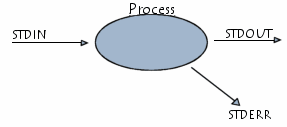
\includegraphics[width=0.65\textwidth]{variaveis/fluxo_shell.jpg}
	\caption{Fluxos de entrada e saída durante a execução de um comando. Imagem obtida de \cite{Shell}}
	\label{fluxo_shell}
\end{figure}



Por padrão, quando se executa um programa, os dados são lidos a partir do teclado e o programa envia a sua saída e os seus erros para a tela. No entanto, também é possível ler os dados a partir de qualquer dispositivo de entrada, ou mesmo a partir de um arquivo, e enviar a saída para um dispositivo de visualização, arquivo etc. Mais informações podem ser obtidas em \cite{Shell}

\section{Compilando e instalando projeto de software}

O Shell, como já explicado, possui a função de executar comandos. Com a finalidade de automatizar a execução de um certo conjunto de comandos, existe disponível no ambiente Linux a ferramenta shell script. Segundo \cite{script}, ''um shell script permite encadear comandos para solucionar tarefas mais complexas, como automatizar backups, redimensionar um lote de fotografias, limpar erros de um arquivo de texto, etc. Mas eles não são apenas uma simples sequência de comandos e podem usar características comuns às linguagens de programação, como condições (if-then-else) e até loops (for, repeat)``.

Neste projeto, criou-se dois shell scripts denominados \textit{build.sh} e \textit{install.sh}. O primeiro, possui a funcionalidade de compilar todo o código fonte já descrito nos capítulos anteriores do ProVANT Simulator. Já o segundo, além de compilar o projeto, ele cria e registra variáveis de ambiente locais (serão descritas na próxima seção) e cria um link simbólico para fácil execução do sistema via terminal. Detalhes sobre os comandos utilizados nos scripts estão explicitados nos mesmos através de comentários.

\section{Variáveis de ambiente}

As variáveis de ambiente são espaços de memória responsáveis por armazenar informações pontuais do sistema. As variáveis podem ser variáveis locais ou variáveis globais. Os nomes das variáveis podem ser constituídos de quaisquer caracteres alfanuméricos (\cite{VE2}). 

Um caso representativo da importância das variáveis de ambiente é o caso da variável de ambiente PATH. A variável PATH é utilizado muitas vezes para se registrar a localização de arquivos executáveis permitindo que o usuário e outros programas possam usufruir de suas funcionalidades.

No caso do ProVANT Simulator, utiliza-se as variáveis de ambiente do ROS e as variáveis de ambiente próprias criadas durante a instalação do sistema. Nesta seção será explicitada apenas sobre as variáveis de ambiente customizadas, sendo que detalhes sobre as variáveis de ambiente do ROS podem ser encontradas em na pagina \url{http://wiki.ros.org}. 

As seguintes variáveis foram criadas:

\begin{itemize}
	\item \textbf{PROVANT\_ROS}: Diretório onde está localizado o código fonte do espaço de de trabalho do usuário no ROS
	\item \textbf{TILT\_PROJECT}: Diretório onde está todo o projeto do ProVANT Simulator 
	\item \textbf{TILT\_STRATEGIES}: Diretório onde está localizado as bibliotecas dinâmicas compiladas com as estratégias de controle de ambiente de simulação
    \item \textbf{TILT\_MATLAB} Diretório onde os arquivos com dados da simulação são
    armazenados
    \item \textbf{PROVANT\_DATABASE}: Diretório onde se encontra os arquivos de descrição de modelos e cenários
    \item \textbf{GAZEBO\_MODEL\_PATH}: Este é uma exceção, não é uma variável ambiente criado, mas sim a atualização de uma variável ambiente do Gazebo. Aqui se encontram os modelos dos VANTs para serem adicionados em simulação.	
\end{itemize}


\bibliography{telefonia/variaveis}